\section{Decentralized Unstructured Algorithms}
\label{section:unstructured}

This section is dedicated to the unstructured P2P architectures. In the next
paragraphs,algorithms for tackling the topology mismatch problem on such
networks are visited, analysed and categorised based on the use of the overlay
structure, messaging approach for peer communication and techniques proposed for
detecting proximity in order to optimise overlay topology. In short, the methods
that are highlighted here are divided into
\begin{inparaenum}[\itshape i\upshape)]
  \item broadcast-based,
  \item cache-based,
  \item overlay optimisation-based, and
  \item landmark-based
\end{inparaenum}
 approaches.

% TODO: READ A Near-Optimal Algorithm Attacking the Topology Mismatch Problem in
%Unstructured Peer-to-Peer Networks (This is an Approximation alg for Top-mis
%problem)

%{\sethlcolor{yellow}\hl{
%HA: TALK ABOUT GNUTELLA HERE!!!!}}

%%%%%%%%%%%%%%%%%%%%%%%%%%%%%%%%%%%%%%%%%%%%%%%%%%%%%%%%%%%%%%%%%%%%%%%%%%%%%%%%
%%%%%%%%%%%%%%%%%%%%%%%%%%%%%%%%%%%%%%%%%%%%%%%%%%%%%%%%%%%%%%%%%%%%%%%%%%%%%%%%
\subsection{Broadcast Based}
%%%%%%%%%%%%%%%%%%%%%%%%%%%%%%%%%%%%%%%%%%%%%%%%%%%%%%%%%%%%%%%%%%%%%%%%%%%%%%%%
%%%%%%%%%%%%%%%%%%%%%%%%%%%%%%%%%%%%%%%%%%%%%%%%%%%%%%%%%%%%%%%%%%%%%%%%%%%%%%%%

In the first realisation of the Gnutella protocol, each query request received
by a peer is then forwarded to all its neighbours, clearly generating
unnecessary traffic over the network. The algorithms highlighted in this
paragraph are referred to as broadcast-based because they enhance the "naive"
broadcasting approach described above and prefer forwarding messages to a
selected subset of a node's outgoing links. The selection criteria vary
depending on the algorithm but they mainly use one or multiple statistical
metrics that span from the obvious ones, like the latency of the link between
the nodes, to more sophisticated alternatives (that may even take into account
application level requirements) such as the reliability of the neighbour. The
forwarding-based approach has the advantage of enhancing search efficiency but
on the other hand suffer drawbacks like the drastic reduction of the search
scope because of the restrictions of the broadcasting policies as well as
limitations when scaling to large networks.

%Expanding the search scope, on the other hand, is no easy task
%because the overhead of forming multicast trees is proportional to the
%multicast group size.
%forwarding based schemes do not consider dynamic joining
%and leaving of peers so they do not scale well on dynamic environments.

%%%%%%%%%%%%%%%%%%%%%%%%%%%%%%%%%%%%%%%%%%%%%%%%%%%%%%%%%%%%%%%%%%%%%%%%%%%%%%%%
\paragraph*{\bf Improving search in peer-to-peer networks}

\begin{figure}[ht]
\centering
\subfigure[Iterative deepening with three levels.] {
  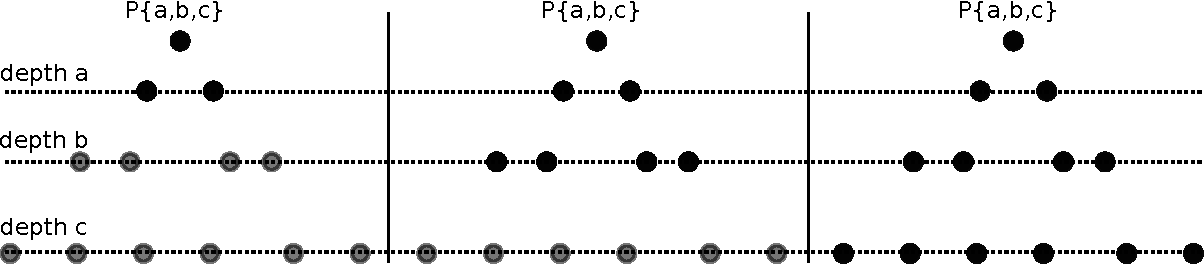
\includegraphics[scale=0.4]{img/algorithms/iterative_deepening}
  \label{figure:dbfs:iterdeep}
}\qquad\qquad
\subfigure[Directed BFS.] {
  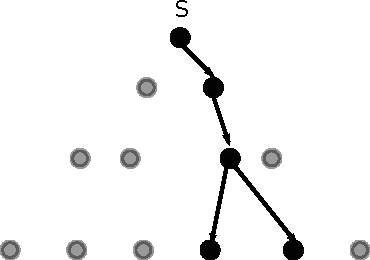
\includegraphics[scale=0.4]{img/algorithms/directed_bfs}
  \label{figure:dbfs:dbfs}
}\qquad\qquad
\subfigure[local indices with radius size equal to $2$.] {
  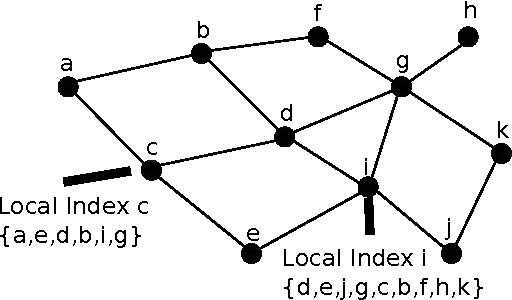
\includegraphics[scale=0.4]{img/algorithms/local_indices}
  \label{figure:dbfs:localindx}
}
\caption{}
\label{figure:dbfs}
\end{figure}

\cite{yang_improvep2psearch_2002} proposes an easy to implement and practical
solution to the inefficiency problem caused by blind flooding in Gnutella-like
P2P file sharing protocols. The paper replaces blind flooding with three
approaches, namely \textit{iterative deepening}, \textit{directed BFS}, and
\textit{local indices}. In \textit{iterative deepening}, as shown in
Figure~\ref{figure:dbfs:iterdeep}, the search is performed on a BFS tree with
multiple preset depths. The depth limit is iteratively increased by the source
node for each query based on the quality of the results. The source node, after
examining the results, may issue a new request by increasing the depth limit,
which will trigger the nodes at the last depth level to resume the search. The
iterative approach avoids to start the search from scratch at each iteration and
reduces the load of the nodes on the upper levels of the tree. The major
drawback of \textit{iterative deepening} is the delay between successive
iterations, as the source node needs to examine the results at each iteration
before deciding to quit or resume the query.  The \textit{directed BFS}, as
shown in Figure~\ref{figure:dbfs:dbfs}, tries to avoid this delay by
forwarding the query messages only to a selected set of neighbours, in which the
selection criteria varies from the number of results received previously,
distance in terms of hops, bandwidth, or the query load of the neighbour. In
\textit{local indices}, as shown in Figure~\ref{figure:dbfs:localindx}, each
node sustains a local data index of the nodes within a radius of $r$ hops from
itself and uses this local index to remotely query the neighbour nodes without
generating additional traffic. \textit{Local indices} greatly reduces the
aggregate bandwidth usage of the network and improves query efficiency, however,
updating the indices in cases with frequent node joins and leaves introduces a
serious overhead to the system if the radius is kept broad.

%%%%%%%%%%%%%%%%%%%%%%%%%%%%%%%%%%%%%%%%%%%%%%%%%%%%%%%%%%%%%%%%%%%%%%%%%%%%%%%%
\paragraph*{\bf Gia}
\emph{Gia} \cite{chawathe_gia_2003} is an effort to solve the scalability
problem of the unstructured P2P file sharing systems, in particular Gnutella.
The main novelty in the design of Gia is the replacement of the blind flooding
approach of Gnutella with random walks \cite{lv_randomwalks_2002}. Although
random walks is a step in the right direction, issuing only a single copy of the
query within the network reduces the search scope, thus affecting negatively the
success rate of the query.  In order to overcome this limitation, Gia introduces
a token-based flow control mechanism, which is essentially an intelligent flow
control algorithm that gradually redirects the queries to nodes which are more
likely to answer. In order to prevent overloading of nodes with query requests,
Gia uses a token-based flow control algorithm in which each node announces the
number of query requests it can handle in terms of tokens to its neighbours, so
that neighbours only forward query requests to nodes that they previously
received tokens from. Gia also acknowledges the heterogenity in peer bandwidth,
processing power, disk speed, etc, of the nodes in P2P networks and uses this
information when connecting nodes to each other and by using a topology
adaptation algorithm, Gia ensures that high capacity nodes have high degrees and
low capacity nodes are within short proximity to high capacity ones. Although
the topology adaptation algorithm Gia uses improves the scalability of the
network, it does not help much in solving the topology mismatch problem, since
it does not consider the underlying physical topology.

%%%%%%%%%%%%%%%%%%%%%%%%%%%%%%%%%%%%%%%%%%%%%%%%%%%%%%%%%%%%%%%%%%%%%%%%%%%%%%%%
\paragraph*{\bf Distributed Cycle Minimization Protocol}
We have already mentioned Gnutella's inefficient broadcasting mechanism in
flooding messages across the network with no actual targeting. This leads, to
nodes that are far from the path towards the query request gratification, to
spend their valuable resources to receive, queue and process messages that they
shouldn't have received in the first place and eventually simply forward them
blindly to continue this vicious cycle. Except from that, though, an other case
of wasting network resources is when a node that is on the right path for the
query, receives the same message multiple times from different neighbours. The
reason for these duplicate messages is cycles in the forwarding paths. Actually,
this duplicate packet problem seems to hurt more the active nodes; those with
higher capacities and bandwidth that contribute the most to the network.
Distributed Cycle Minimization Protocol (DCMP) \cite{zhu_dcmp_2008} introduces a
method to
remove the cycles and eliminate the duplicate packets, without sacrificing
overlay connectivity. In DCMP, once a cycle is detected, the most powerful node
in the cycle is elected as the \emph{Gate Peer} and the cycle is then destroyed
by cutting that special link which will result in the minimisation of the
distance to the Gate Peer for all the nodes that participated in that cycle. The
process is managed by using two special message types namely \emph{Information
Collection (IC)} and \emph{Cut Message (CM)}. One disadvantage of DCMP is that
since the distance a forwarded message can travel is limited by the TTL value,
which is practically $7$ in most cases DCMP cannot detect cycles formed by more
than 7 peers. Even though cycle elimination improves the network performance, it
does not actually solve the topology mismatch problem.

%%%%%%%%%%%%%%%%%%%%%%%%%%%%%%%%%%%%%%%%%%%%%%%%%%%%%%%%%%%%%%%%%%%%%%%%%%%%%%%%
%%%%%%%%%%%%%%%%%%%%%%%%%%%%%%%%%%%%%%%%%%%%%%%%%%%%%%%%%%%%%%%%%%%%%%%%%%%%%%%%
\subsection{Cache Based}
%%%%%%%%%%%%%%%%%%%%%%%%%%%%%%%%%%%%%%%%%%%%%%%%%%%%%%%%%%%%%%%%%%%%%%%%%%%%%%%%
%%%%%%%%%%%%%%%%%%%%%%%%%%%%%%%%%%%%%%%%%%%%%%%%%%%%%%%%%%%%%%%%%%%%%%%%%%%%%%%%

%\subsection{Cache Based}
%
%Caching based protocols are effectively used to reduce traffic costs and
%response
%times. The caching policy varies depending on the way protocol handles the
%index and the
%content. Centralized P2P systems
%use central index servers, while local caching systems, such as KazaA, use
%super peers
%to cache indices in a distributed way. Content caching is also possible in P2P
%systems, where nodes cache the forwarded content for further retrievals.
%Although caching has the above mentioned advantages,  duplication
%of messages still exist, which limits the scalability of these approaches.
%Therefore, cache based approaches are analyzed in the following categories:
%  \begin{itemize}
%    \item \emph{data index caching},
%    \item \emph{content index caching},
%    \item \emph{centralized}, and
%    \item \emph{local}.
%  \end{itemize}
%
Caching is a widely used technique to exploit locality and minimise redundant
transfer of data, initially adopted by web and file server application
environments with great success. Since peers in a P2P system also work as
servers, it is intuitively expected that P2P file sharing systems can also
benefit from caching. However, two of the main characteristic properties of P2P
systems, nodes frequently joining and leaving and query lifetime relatively
short (at least compared to those needed to be served by web servers) , makes
caching in P2P networks a non-trivial issue. There are usually two levels of
caching possible in file sharing systems, caching indices or pointers to data or
caching the data itself. Caching is already implemented and successfully used in
some commercial P2P systems. One popular example is KazaA, which uses caching of
indices on its super-peer level. In the paragraphs below, caching-based
algorithms are presented and explained in more depth.

%%%%%%%%%%%%%%%%%%%%%%%%%%%%%%%%%%%%%%%%%%%%%%%%%%%%%%%%%%%%%%%%%%%%%%%%%%%%%%%%
\paragraph*{\bf Replication Strategies in Unstructured Peer-to-Peer Networks}
\cite{Cohen02} aim to improve the inefficient blind search algorithm by
replicating the data in a P2P network. The main intuition behind the
idea of replication, or using cached copies, is that as the number of copies for
each item increases in the network, it would be easier for a search algorithm,
even a random one, to locate these items. In order to analyse the feasibility of
such an approach, the authors investigate three different replication
strategies, namely uniform, proportional, and square root allocation. In the
uniform model, the copies of items are uniformly replicated in the network,
while in the proportional model, the items are replicated based on their query
rate, so that frequently queried items are replicated more. The square root
allocation is a strategy proposed in this paper, which is a model between the
uniform and proportional allocation.  In order to evaluate the outcome of the
replication models, the overall costs of successful and unsuccessful searches in
the network are compared. Results argue that the uniform allocation model
minimizes the maximum search size, therefore reduces the time spent on an
unsuccessful search. The proportional model, on the other hand, promotes the
more frequently queried items by replicating them more, therefore decreases the
search time for popular items, but suffers when needing to locate the rare
items. The authors also claim that the expected successful search size is the
same for uniform and proportional models, and any approach between them would
behave much better. Therefore they propose the square root allocation approach,
which is a replication strategy that minimizes the expected search size of
successful queries in P2P networks.

%%%%%%%%%%%%%%%%%%%%%%%%%%%%%%%%%%%%%%%%%%%%%%%%%%%%%%%%%%%%%%%%%%%%%%%%%%%%%%%%
\paragraph*{\bf Tracing a large-scale Peer to Peer System: an hour in the life
of Gnutella}
\cite{Markatos02} analyses Gnutella network traffic traces and by concluding
there is locality among query requests, proposes a caching algorithm that tries
to exploit these findings . The analysis of the trace data reveals other
important facts about the structure of the Gnutella network and the query data.
One significant observation is that the geographic locations of clients do not
have a correlation with the number of query requests they receive. This is an
obvious result of the topology mismatch problem caused by the overlay structure
of the Gnutella network. Gnutella's traffic is observed to be bursty both for
query requests and query responses, even in longer intervals. It is observed
that a peer receives 50 query messages per second on average! Moreover nine out
of ten queries do not generate any response due to the inefficient design of
the Gnutella network. When developing a caching system to exploit locality,
applying an approach similar to web caching does not fit well with P2P systems.
Caches in P2P systems not only have to consider the query string, but also
the TTL value, the source of the query, and the time of the query as well.  In
general, even though optimum caching is hard to achieve, it is reported that
it improves the overall performance of the Gnutella network.

%%%%%%%%%%%%%%%%%%%%%%%%%%%%%%%%%%%%%%%%%%%%%%%%%%%%%%%%%%%%%%%%%%%%%%%%%%%%%%%%
%%%%%%%%%%%%%%%%%%%%%%%%%%%%%%%%%%%%%%%%%%%%%%%%%%%%%%%%%%%%%%%%%%%%%%%%%%%%%%%%
\subsection{Overlay Optimization Based}
%%%%%%%%%%%%%%%%%%%%%%%%%%%%%%%%%%%%%%%%%%%%%%%%%%%%%%%%%%%%%%%%%%%%%%%%%%%%%%%%
%%%%%%%%%%%%%%%%%%%%%%%%%%%%%%%%%%%%%%%%%%%%%%%%%%%%%%%%%%%%%%%%%%%%%%%%%%%%%%%%

The overlay optimization based protocols modify the topology of the P2P network
using various techniques. The two commonly used approach that is investigated in
this section are creating spanning trees using connection graphs, and creating
clusters of physically close nodes. Spanning tree based approaches construct
rich graphs based on the network connections and build minimum spanning trees on
these graphs. Even though spanning trees provides efficient query performance,
the construction and the update costs of the spanning tree, especially in
dynamic environments with many nodes joining and leaving the network, cause
large traffic overhead to the corresponding
network \cite{chu_esm_2000,chu_esm_2002}. The cluster based approaches on the
other hand select to link physically closer nodes with each other, therefore
significantly shrinking the search scope of the system. Added to that, commonly
used methods for correct determination of physical node positions across
Internet do not always return reliable results, therefore mapping accuracy is
not guaranteed. Bellow, the details of the algorithms that use the spanning tree
based or cluster based topology optimization methods are presented.

%%%%%%%%%%%%%%%%%%%%%%%%%%%%%%%%%%%%%%%%%%%%%%%%%%%%%%%%%%%%%%%%%%%%%%%%%%%%%%%%
\paragraph*{\bf Narada}

\begin{figure}[ht]
\centering
\subfigure[Underlying network with edge costs.] {
  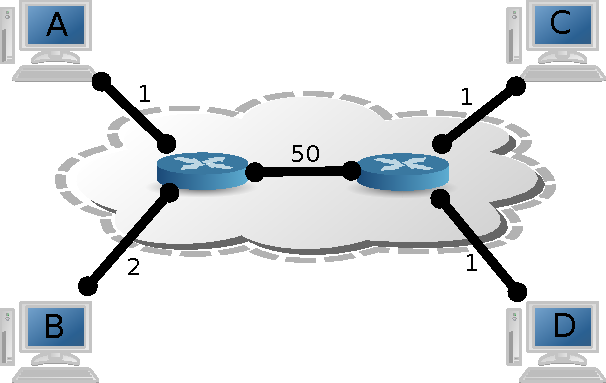
\includegraphics[scale=0.4]{img/algorithms/narada}
  \label{figure:narada:underlying}
}\qquad\qquad
\subfigure[Peer A sends a message to the rest using regular broadcast.] {
  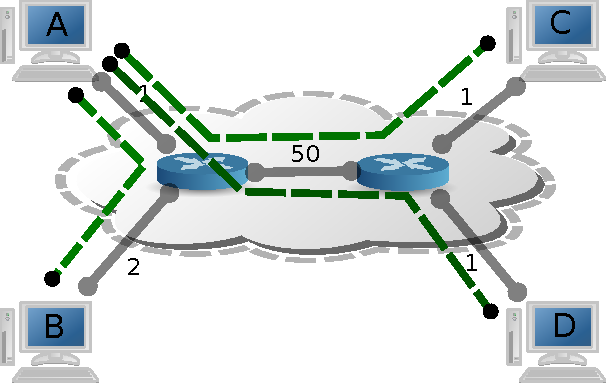
\includegraphics[scale=0.4]{img/algorithms/narada2}
  \label{figure:narada:regu}
}\qquad\qquad
\subfigure[Peer A sends a message to the rest using end system multicast.] {
  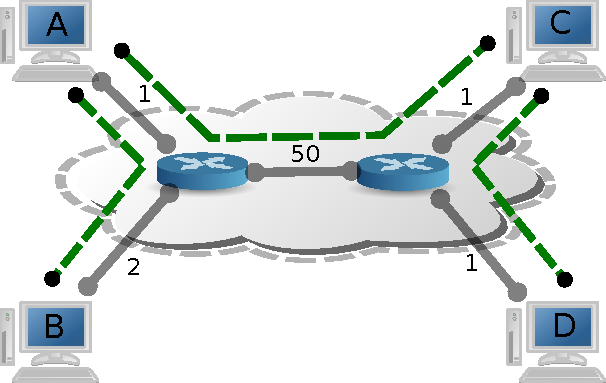
\includegraphics[scale=0.4]{img/algorithms/narada3}
  \label{figure:narada:multicast}
}
\caption{A visualisation of the Narada protocol.}
\label{figure:narada}
\end{figure}

Narada \cite{chu_esm_2000,chu_esm_2001,chu_esm_2002} is a generic protocol for
creating self-adapting overlay networks, that can achieve application-layer
multicast communication without requiring IP multicast infrastructure at the
network layer. IP multicast is the term reffering to the method of sending IP
datagrams to a group of receivers in a single transmission. Even though the
method is available some years now, IP multicast has not taken off as
anticipated since many believe that it violates the stateless design of the
current Internet. For this reason it is widely deployed in contained
environments like enterprises (i.e. IPTV applications - distance learning, video
conferencing), commercial stock exchanges, and multimedia content delivery
networks. Narada tries to break these constraints. Although it was not
originally designed as a P2P file sharing protocol, it has become one of the
pioneering works in the overlay networks area. The authors claim that, although
Narada is not as efficient as IP multicast, still it provides reasonable
performance, without the additional cost of implementing multicast services on
the current Internet infrastructure. Additionally, authors realised the
inefficiency caused by the topology mismatch problem and tried to encounter it
by building a richer connected graph, called a mesh, and building per source
minimum spanning trees \footnote{ENarada \cite{li_enarada_2008} used Gossip
protocol for the construction} as shown in Figure~\ref{figure:narada}. They also
keep the graph and the trees dynamically updated while nodes continue to join
and leave the network. Moreover, the protocol tries to ease the physical link
stress, the overall resource usage and the relative delay among end systems.
Unfortunately, the most imporpant limitation of Narada is that although it works
reasonably well for small groups, it does not scale well for larger networks,
therefore it is not suitable for, potentially very large, P2P file sharing
application networks.

%%%%%%%%%%%%%%%%%%%%%%%%%%%%%%%%%%%%%%%%%%%%%%%%%%%%%%%%%%%%%%%%%%%%%%%%%%%%%%%%
\paragraph*{\bf Adaptive Overlay Topology Optimization and Adaptive Connection
Establishment}
\emph{Adaptive Overlay Topology Optimization (AOTO)} \cite{liu_auto_2003} is one
of the first attempts, along with Narada, from the P2P research community to
address the topology mismatch problem. AOTO is a distributed algorithm that uses
\emph{Selective Flooding} and \emph{Active Topology} to optimize the overlay
network topology. The \emph{Selective Flooding} algorithm creates a minimum
spanning tree over the overlay and uses this tree instead of flooding the whole
network, without shrinking the search scope. In \emph{Active Topology}, the
physical locations of nodes are estimated based on the network delay among them
and physically close nodes are connected as neighbours to revise the overlay
topology as close as possible to the physical network topology. Overall, AOTO
reports a $55\%$ performance improvement in terms of the traffic load. In
\emph{Adaptive Connection Establishment (ACE)} \cite{liu_ace_2004}, the authors
extend the idea by introducing optimizations based on the depths of the minimum
spanning trees. But since the network delay is not always a reliable estimation
method to detect the physical location of peers, the algorithm still suffers
from the discrepancies caused by mislocated nodes.

%%%%%%%%%%%%%%%%%%%%%%%%%%%%%%%%%%%%%%%%%%%%%%%%%%%%%%%%%%%%%%%%%%%%%%%%%%%%%%%%
\paragraph*{\bf Location-aware Topology Matching}
\emph{Location-aware Topology Matching (LTM)} \cite{liu_ltm_2004} proposes a
method to optimize the overlay structure of the P2P network based on the
physical topology. To achieve this, the algorithm issues a special message
called \textit{TTL2-detector} to detect the latency of two-hop neighbours
($N^2$) around each node. The latency information gathered is later used to
evolve the overlay network into a more efficient one, without reducing the
search scope. Each node examines the latency information with the neighbours and
low productive connections are dropped and replaced by more efficient ones, thus
reducing the latency on the overall network, and eliminating some potential
inefficiencies, such as unnecessary crossing of messages over autonomous system
(AS) boundaries, etc. Although LTM improves the overall efficiency of the P2P
network, it does not actually use real physical topology information, just
latency metrics, therefore it does not offer a guaranteed safety net for the
topology mismatch problem.

%%%%%%%%%%%%%%%%%%%%%%%%%%%%%%%%%%%%%%%%%%%%%%%%%%%%%%%%%%%%%%%%%%%%%%%%%%%%%%%%
\paragraph*{\bf Scalable Bipartite Overlay}
\emph{Scalable Bipartite Overlay
(SBO)} \cite{liu_bipartite_IPDPS,liu_bipartite_2007} reduces the overhead of
creating and maintaining a minimum spanning tree cost by randomly dividing the
nodes into two groups, namely red and white and assigning different tasks to
different groups. The white peers measure distances to neighbours by using the
network delay as the metric and reports the results to red peers. The red peers,
equipped with the information of all two-hop neighbours ($N^2$), creates a
minimum spanning tree of these neighbours and assigns efficient forwarding
paths. The white peers can further optimize their positions within the overlay
if this is required.

%%%%%%%%%%%%%%%%%%%%%%%%%%%%%%%%%%%%%%%%%%%%%%%%%%%%%%%%%%%%%%%%%%%%%%%%%%%%%%%%
% TODO: DOUBLE CHECK IF THIS ALGORITHM GOES IN THIS SECTION/SUBSECTION
\paragraph*{\bf Adaptive Peer Selection}
Bernstein et al., contributed on the use of machine learning for building peer
selection strategies from past experience \cite{bflz_adaptpeersel_2003}. A
decision tree is used to rate peers based on information about connection
characteristics that is collected. These can be load, bandwidth, and past
uploading experience. Then a by Markov decision process is incorporated as a
mechanism to shape the policy for switching among the peers. The problem
with this approach is that the peer selection algorithm is slow due to the
learning process and the complexity of the method.

%%%%%%%%%%%%%%%%%%%%%%%%%%%%%%%%%%%%%%%%%%%%%%%%%%%%%%%%%%%%%%%%%%%%%%%%%%%%%%%%
\paragraph*{\bf Innocuous Topology Aware (ITA) Overlay Construction}
\cite{prfm_ita_2009} intoduces an algorithm for Innocuous Topology Aware
construction of unstructured P2P networks. The paper's proposition is twoforld.
Overlay construction and search method. For the overlay construction it employs
the notion of \emph{short} and \emph{long} connections. Assuming $N$ is the
number of all network participants, $\alpha \leq 1 $ a system-wide magic number
and $x$ an $\alpha$-related latency threashold, the bootstrapping peer randomly
selects $\alpha \ast N$ close (latency bellow $x$) and
$\left( 1 - \alpha \right) \ast N$ distant (latency above $x$) nodes as its
neighbours. The search method has two steps. First, the quering node initiates a
flood to its distant neighbourhood with $TTL = 1$. Then, peers that receive a
query over a long link, start a local flood with $TTL = ttl$, were $ttl$ is a
system defined parameter.

The goal of the overlay construction is to create a network that exposes low
clustering, a beneficial characteristic of random graphs which can lead to a
larger coverage of peers with the same number of messages and reduced
duplication. This means more efficient information lookup that exposes low or no
negative impact whatsoever to the rest of the mechanisms employed in
unstructured P2P systems\footnote{For example the 1-hop replication and the
dynamic querying mechanisms of later versions of Gnutella.}. The paper reports
50\% reduction in communication latency ammong peers by cutting off some 20\% of
the IP-level message traffic generation.

%%%%%%%%%%%%%%%%%%%%%%%%%%%%%%%%%%%%%%%%%%%%%%%%%%%%%%%%%%%%%%%%%%%%%%%%%%%%%%%%
\paragraph*{\bf EGOIST}
EGOIST \cite{egoist_2008} is a set of algorithms to construct and manage overlay
networks. It utilises a selfish approach in the sense that every participating
peer continuously updates its neigbours so as to minimise the sum of distances
to all destinations under shortest-path routing. In EGOIST, a newlly arriving
peer, randomly connects to an already participating node through a bootstrap
server. Being connected, it starts receiving info throught the link-state
mechanism and thus, after some time, it has a complete picture of the overlay
graph. Then it estimates the delay to all other nodes in order to determine its
potential neighbours and ultimatelly connect to the overlay using some
policy\footnote{For example, minimisation of the average delay to all its
neighbours.}. It is obvious that there is extensive resource usage for updating
the wiring of the all nodes in the system. The authors claim that they can
reduce the load imposed by the monitoring and announcing process from $O(n^2)$
to only $O(kn)$, where $n$ is the number of all nodes in the network and $k$ is
the number of links a node chooses to establish.

% TODO: CHECK IF THE FOLLOWING BITTORRENT ALGORITMS BELONG IN THIS SUBSECTION
%%%%%%%%%%%%%%%%%%%%%%%%%%%%%%%%%%%%%%%%%%%%%%%%%%%%%%%%%%%%%%%%%%%%%%%%%%%%%%%%
\paragraph*{\bf Biased Neighbour Selection}
Bindal et al. \cite{rpc_bitbiased_2006} claim to strengthen BitTorrent
protocol\cite{c_bittorrent_2003} locality by selecting most of a peer's
neighbours to be out of the same ISP, while preserving the near optimal download
performance of the protocol itself. BitTorrent systems employ most of the time
mechanisms that can be proven very aggresive to an ISP's networking and
accounting, basically, due to their lack of knowlegde of AS boarder limits.
BitTorrent specification, by default allows for each peer, 35 connections.
Biased neighbour selection experiments on some number $k$ which denotes a number
of neighbouring peers which are not on the same ISP than the peer at hand.
Consequently, the remaining $35 - k$ peers are from the same ISP. These $k$
nodes are used in order to preserve a more extended, global view of a network,
but in the same localize the load within the limits of a single ISP. This
prevents clients from exchanging traffic through an expensive transit link, if
there are alternative local connections that could offer the same, faster and at
no additional cost for the ISP. Implementation can either be done through
modifications on the tracker side, to identify ISP locallity, or through P2P
traffic shaping devices installed on ISP's edge routers. The paper also proposes
combination of biased neighbour selection along with bandwidth throttling and
some caching approach for near optimal results. Unfortunatelly, implementation
need, in some extend, contribution (exposure of ISP AS mappings) or
infrastructure changes (installation of P2P traffic shaping devices) on the ISP
level itself, making the adoption difficult in the general case.

%%%%%%%%%%%%%%%%%%%%%%%%%%%%%%%%%%%%%%%%%%%%%%%%%%%%%%%%%%%%%%%%%%%%%%%%%%%%%%%%
\paragraph*{\bf Ono}
Choffnes and Bustamante propose Ono \cite{cb_ono_2008}, a protocol for managing
BitTorrent traffic so that it significantly reduces cross-ISP traffic and in
the same time enhances downloading rates by favouring connections within the
borders of a single autonomous system. Contrary to biased peer selection
proposed in \cite{rpc_bitbiased_2006}, this work can lead to improved
performance with no cooperation between ISPs and their subscribers, no
additional infrastructure and no network topology information. The selection
approach is landmark-based and leverages existing CDN infrastructure for peer
distance estimation. CDNs already use both static (i.e. geographical) and
dynamic (network measurement systems) information for their replica selection,
so the authors claim that peers which exhibit similar redirection behaviour, are
very likely they are close to the replica servers and as a consequence to each
other. The redirection behaviour is modeled in terms of \emph{ratio map} in the
article's parlance, a vector of (replica-server,ratio) tuples, where ratio is
the percentage of times CDN redirects the peer to the specific replica-server.
The bootstrapping phase consists of the peer performing DNS lookup to CDN names
in order to build its redirection information. The interval for polling DNSs
starts from 30 seconds and increases by one minute every time redirection info
to the CDN is found to remain unchanged after a lookup. On the other hand, the
interval is halved whenever is found to have been changed. In order not to avoid
the bootstrapping phase if the ratio map is sufficiently fresh, the protocol
persists the info after the end of a BitTorrent session.

%%%%%%%%%%%%%%%%%%%%%%%%%%%%%%%%%%%%%%%%%%%%%%%%%%%%%%%%%%%%%%%%%%%%%%%%%%%%%%%%
\paragraph*{\bf Locality-Awareness in BitTorrent-like P2P Applications}
In \cite{lclx_bitlocal_2009} the authors study and compare three different
approaches in injecting locality awareness in BitTorrent-like applications. The
first acts at a \emph{macroscopic-level} and targets neighbour selection. When a
peer asks the tracker to join, the later sorts the swarm peers according to
their distance to the requesting peer in AS hop count and send it the first
(e.g. 50) peers in the list. The second manipulates the chocking/unchocking
BitTorrent mechanisms at an \emph{intermediate-level}. A peer unchockes its 4
closest in terms of AS hop count interested neighbours. The same applies also
when the peer turns to the seeding state\footnote{Thus this approach favours
least distance, contrary to the original BitTorrent implementation which favours
uploading speed.}. On a \emph{microscopic-level}, the rare-first chunk picking
policy is substituted by the locality-fist policy. The distance value of a piece
is calculated as the mean value of the distances of the peers that posses it.
The paper conducts several measurements on the efficiency of the above scheme to
reach the conclusion that the major design desision for all locality aware P2P
systems is the trade-off of optimising inter-AS traffic, which their solution
achieves, and of the fairness among peers, a section that their locality-based
approach does not do well in comparison to the random approach of the standard
BitTorrent protocol.

%%%%%%%%%%%%%%%%%%%%%%%%%%%%%%%%%%%%%%%%%%%%%%%%%%%%%%%%%%%%%%%%%%%%%%%%%%%%%%%%
\paragraph*{\bf TopBT}
\cite{rtlcgz_topbt_2010} proposed an approach for enhancing proximity awareness
in the BitTorrent protocol without any need of any infrastructure installed. It
suggests that a good peer selection metric should take into account both the
downloading speed and the network topology. Thus, it proposes the use of the
ration of download rate to upload rate, $\frac{d}{u}$, divided by link-level or
AS-level routing hops, $l$ or $a$ respectively, in an attempt to form a
comprehensive metric to select peers with high download rate, low reciprocal
upload demand and low routing hops. The TopBT metric is applied on serveral
parts of the original BitTorrent protocol in order to inject topology awareness
for better peer selection; more specifically on the peer list the tracker
returns when someone first tries to connect to the swarm, on the initial
connection establishment on the connection replacement and of course the
unchoking mechanism.

%A peer that runs the TopBT protocol evaluates its neighbours by periodicaly
%emitting pings or traceroutes in order to uchock those peer that exhibit less
%hops to reach and higher download rates. \emph{Link-hops} are measured by using
%the TTL value that the originator receives as a response from the remote
%peer\footnote{Initial TTL values are known for the different operating systems
%(e.g. 64 for Linux or 128 for Windows NT/2000/XP) so the originator can
%calculate the hops using the value of the TTL on the response message it
%receives.}. Also the peer, when offline, builds a table that maps IPs to
%\emph{AS-hops}, using BGP dumps.

Through experimentation on hundreds of PlanetLab as well as residential hosts,
the authors claim more than 25\% traffic reduction and 15\% faster downloads,
both with a lightweight cost when compared to popular BitTorrent
implementations.

%%%%%%%%%%%%%%%%%%%%%%%%%%%%%%%%%%%%%%%%%%%%%%%%%%%%%%%%%%%%%%%%%%%%%%%%%%%%%%%%
\paragraph*{\bf Underlying Topology-Aware Peer Selection (UTAPS)}
UTAPS \cite{lcy_utaps_2008} is another peer selection strategy for the
BitTorrent protocol. Its first step is to collect the needed information in
order to construct a picture of the underlying topology and the second is to
make the peer selection, per se, based on this knowledge. For the first part,
the algorithm uses network tomography, a technique which suggests probing only
from a large network's end points in order to infer its internal characteristics
\cite{chny_tomography_2002}. Upon a new peer arrival, the tracker traceroutes it
to get some knowledge (IP address, routers involved, RTT and hops conducted
e.t.c). The more the peers in the swarm the better picture a tracker has for the
underlying infrastructure, which can then return to the newcomming peer in the
form of the bootstrapping peer list. The peers furtherly enhance this picture by
tracerouting the returned peers themselves and reporting back to the tracker.
For the selection part, a family of heuristics are proposed, which in general
target those peers that expose low RTT and are within certain hop-count away of
measured routers. The author's claim that peers running UTAPS instead of random
peer selection can achieve better downloading rates with reduced burden on the
underlying ISP infrastructure though their technique is coarse-grained and their
evaluation configuration was far too small for extracting further safe
conclusions.

%%%%%%%%%%%%%%%%%%%%%%%%%%%%%%%%%%%%%%%%%%%%%%%%%%%%%%%%%%%%%%%%%%%%%%%%%%%%%%%%
\paragraph*{ \bf An Effective Network-Aware Peer Selection Algorithm in
BitTorrent}
Qin et al., in their work in \cite{qlzg_biteffpeersel_2009}, propose a
clustering approach that differentiates peers in a swarm into local, intra-ISP
and inter-ISP neighbours. The classification is done through the routers they
use in order to communicate with the tracker. For this, a newly arriving
BitTorrent peer traceroutes the tracker and sends the results in a form of a
vector of triples that contain the IP and the hop counter for the router on the
traceroute path as well as the link latency of the hop that was made in order to
arrive to this router. The tracker uses this information in order classify the
router through a $k$-means classification algorithm, with $k = 3$. For peer
selection, the authors propose a biased approach where the tracker returns $c$
close peers and $d = N - c$ distant peers, where $N$ is the length of the
returned list. In choosing $c$, the tracker employs an iterative search process
first in the peer's local neighbourhood. If not enough peers are available
there, it goes to intra-ISP and subsequently, if needed, to the inter-ISP
cluster. The evaluation of the algorithm is done in a similar artificial,
contained laboratory enviromnent as in \cite{lcy_utaps_2008} and it shows up to
5\% faster downloading times, and up to 22\% reduction of the total cross-ISP
traffic.

%\paragraph*{\textbf{Two-Hop-Away Neighbour Comparison and Selection\\}}
%
%\paragraph{}
%Work in \cite{liu_thancs_2005,liu_thancs_2008} proposes a distributed heuristic
%called \emph{Two-Hop-Away Neighbour Comparison and Selection (THANCS)} that
%\begin{inparaenum}[\itshape i\upshape)]
%  \item is completely distributed and needs no global knowledge,
%  \item presents trivial overhead compared to the query cost savings
%  \item its convergent speed of the algorithm is fast enough (faster than
%minimum spanning tree approaches) so that is effective to dynamic environments,
%and
%  \item does not shrink the search scope.
%\end{inparaenum}
%
%\paragraph{}
%THANCS is considered a \emph{local search method}, in the sense that it targets in finding a locally optimum solution, by exploiting knowledge within a 2-hop radius. The algorithm consists of two main components: \emph{piggybacking neighbour distance on queries} and \emph{neighbour comparison and selection} which are furtherly discussed bellow.
%
%\paragraph{Piggybacking neighbour distance on queries}
%Using network delay as a metric for measuring the distance, each peer probes distances with its immediate naighbours and stores information locally. For this reason a special query message type, \emph{Piggy Message (PM)}, is introduced. It is 6 bytes long and includes two fields: Neighbour IP Address and Neighbour Distance. A peer $P$ constructs a PM for its neighbour $Q$, which contains $Q$'s IP address and $Q$'s distance from $P$. When $P$ receives a query from $Q$, this PM will be piggybacked by the query that goes to all other neighbours of peer $P$. Upon receiving such a query message, each of the other neighbours will detach the PM, record the $PQ$ distance and process the query. This PM will not be further forwarded. In selecting which incoming queries  should piggyback a PM the paper proposes the \emph{pure propability-based (PPB)} and the \emph{new neighbour triggered (NNT)} policies.
%
%\paragraph{Neighbour comparison and selection}
%Figure~\ref{figure:thancs} illustrates this component of the THANCS algorithm. A peer $S$ probes the distance to all known unprobed $N^2(S)$\footnote{$N^2(S)$ denotes the set of peers being two hops away from $S$, while $N(S)$ denotes the set of direct logical neighbours of $S$.}. The distance of $SP$ is known to $S$. Upon receiving a PM from node $P$ with the distance of $PQ$, $S$ follows one of the following:
%\begin{itemize}
%  \item $Q \in \left( N(S) \cap N^2(S) \right)$, i.e. $Q$ is direct neighbour of $S$. In this case $S$ will compare cost of $SQ$, $SP$ and $PQ$. If the most costly connection is one of $SQ$ or $SP$ the corresponding link will be put into a \emph{will-cut list}\footnote{Links are not immediately disconnected when put in the will-cut list. There are useless for forwarding but are kept active, for some time, in order to serve query responses that are traveling to the source peer along the inverse search path.}. If the most costly connection is $PQ$ then $S$ will do nothing, as the fully distributed nature of the algorithm will give a chance to either $P$ or $Q$ to cut the connection.
%  \item $Q \in \left( N^2(S) - N(S) \right)$, i.e. $Q$ is a two-hop-away neighbour of $S$. If $S$ hasn't probed $Q$ before\footnote{A distance cache is maintained and looked up in such a case.}, it probes and stores the result in the \emph{distance cache}. Having the distance of $SQ$, $S$ compares costs of $SQ$, $SP$ and $PQ$. If $SQ$ is the most costly, $S$ will not establish the connection. If $SP$ is the most costly, $S$ will establish connection $SQ$ and put $SP$ in the will-cut list. If $PQ$ is the longest, $S$ will keep  the connection with both $P$ and $Q$, expecting that $P$ or $Q$ will eventually disconnect link $PQ$, later.
%\end{itemize}
%
%\begin{figure}
%\centering
%  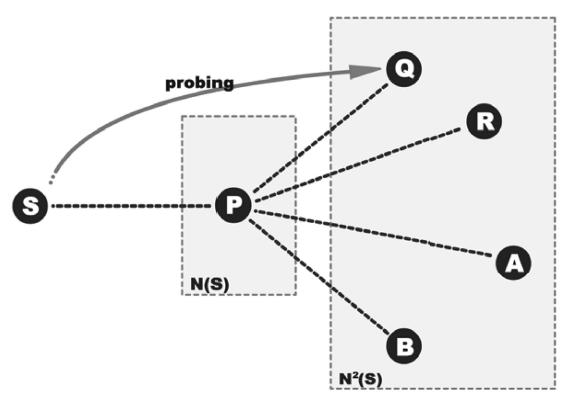
\includegraphics[scale=0.4]{img/thancs.jpeg}
%\caption{Probing two-hop-away neighbours}
%\label{figure:thancs}
%\end{figure}
%
%\paragraph{}
%In a static environment THANCS has been proven to be effective; optimizing 45 percent out of the 60 percent of mismatched paths, constructing a nearly optimal overlay. This leads to a 60 percent reduction in traffic cost as well as a 40 percent decrease in query response time. In dynamic environments (Gnutella 0.6/Limewire super-peer-like and Ion flat-like), THANCS saves up to 70 percent of the traffic cost in the super-peer topology and 55 percent for the flat one. Average response time is also decreased by 60 and 45 percent, respectively. Generally, THANCS has similar performance to LTM, without needing synchronization. SBO, incurring half the  overhead of AOTO, reduces the traffic cost the most, while THANCS has lower response time and converges faster than SBO. THANCS is, thus, more suitable for a more dynamic environment. In addition, THANCS is easy to implement and its operation overhead is trivial, compared with the other three approaches. This design, however, has the limitation of not being easily extend to also support non-flooding-based systems.


%%%%%%%%%%%%%%%%%%%%%%%%%%%%%%%%%%%%%%%%%%%%%%%%%%%%%%%%%%%%%%%%%%%%%%%%%%%%%%%%
\paragraph*{\bf Peer-exchange Routing Optimization Protocols}
\cite{qiu_prop_2007} introduces two protocols called \emph{Peer-exchange Routing
Optimization Protocols (PROP)} to adjust the neighbourhood graph of an overlay
network in order to reduce its overall link latency. PROP algorithms are based
on the exchange of neighbours among peers, driven by the mutual benefit of the
participants to reduce the network delay among their connections.  In PROP-G
(Generic), a peer can exchange all of its neighbours with another peer, while in
PROP-O (Optimized) two peers exchange a selected subset of their neighbours.
PROP-G is a generic protocol that guarantees the connectivity of the overlay
graph during exchanges, therefore can be applied to both unstructured and
structured overlay networks.

%%%%%%%%%%%%%%%%%%%%%%%%%%%%%%%%%%%%%%%%%%%%%%%%%%%%%%%%%%%%%%%%%%%%%%%%%%%%%%%%
\paragraph*{\bf T2MC}
T2MC \cite{shi_t2mc_2008} uses traceroute logs to detect different autonomous
systems and cluster close by peers, thus reducing redundant traffic that crosses
autonomous system boundaries. T2MC uses a customized k-mean classification
algorithm with $k=2$ to perform the classification, and exploits the stable
structure of the Internet routers to guide clustering. Even though traceroute
provides detailed information about the network structure, its excessive use
creates additional overhead that stresses further the overall network
infrastructure. This forces network administrators to disable its support from
the routers they manage, thus jeopardizing the effectiveness of the T2MC
algorithm.

%\paragraph*{\textbf{T2MC\\}}

%\paragraph{}
%\emph{T2MC}\cite{shi_t2mc_2008} exploits some properties of the Internet
%paradigm and clusters nodes belonging to the same ISP without any centralised
%control or predefined system parameterization. The algorithm considers the
%dynamic nature of peers and exploits the stable nature of routers in order to
%build a topology location relationship among end peers.
%
%\paragraph{}
%Some special routers split the physical network into autonomous system domains.
%Using a Traceroute mechanism T2MC searches for latency leaps among the path to
%a host in order to form ``near'' and ``remote'' router clusters. This is
%achieved by a 2-Means Classification, defined by the following steps:
%\begin{enumerate}
% \item the peer chooses the minimum and maximum Latency results from the
%Traceroute for initializing the cntroinds of two sets ``first'' and ``second''.
% \item The peer calculates, for all hops allong its tracerouted path, the
%absolute distance to the centroids of both sets and assigns the routers to that
%centroid with which it has the smaller absolute distance.
% \item The peer calculates the latncy mean and variance value of two sets
% \item If the variance is larger than a predefined threshold then the algorithm
%takes a loop from step 2 picking the two latency mean values as new centroids
%of sets ``first'' and ``second''.
%\end{enumerate}
%Ultimately peer will end up with two sets having the minimum intra-set
%variance. Finally the peer chooses the router from ``second'' set with the
%minimum hops attribute and sets it as a threshold. The selected router and all
%others whose hops attribute is larger than the threshold are classified as
%``remote'' router cluster. The remaining are classified as ``near''. From the
%``near'' class, the peer chooses the one with maximum hops attribute as its
%edge router, and registers it along with the all the ``near'' cluster into the
%DHT of the p2p overlay. As new peers join the network, those that share the
%same edge router or any of the members of the ``near'' router clustersm ther
%would gather to form a ``close'' peer cluster. As Edge routers can provide more
%valuable information than other members of the ``near'' set, T2MC was designed
%to prioritize interaction of peers and edge gateways.
%
%% TODO: figure t2mc.jpeg (a) stars represent edge routers (b) hop leaps
%
%\paragraph{}
%The use of Traceroute as a tool for implementing the distance measuring
%infrastructure raise concearns about its efficiency and scalability. Being,
%primarilly, a network diagnostic utility, it is concearned too heavy weighted
%and intrucive for use in a larger scale\cite{ratnasamy_binning_2002}.
%Additionally, disabling ICMP is a common administrative policy for edge sites
%to enforce security, while dumping BGP routing
%tables\cite{krishnamurthy_bgpclust_2000} is not directly available to the
%application layer.

%%%%%%%%%%%%%%%%%%%%%%%%%%%%%%%%%%%%%%%%%%%%%%%%%%%%%%%%%%%%%%%%%%%%%%%%%%%%%%%%
\paragraph*{\bf Resolving the Topology Mismatch Problem in Unstructured
Peer-to-Peer Networks}
% TODO: to be reviewed

In \cite{hsiao_redblue_2009}, Hsiao et al, claim to construct topology-aware
unstructured overlays that \emph{guarantee} performance qualities in terms of
\begin{inparaenum}[\itshape i\upshape)]
  \item the expected communication latency among any two overlay peers
regardless of the network size, and
  \item the broadcasting scope of each participating peer
\end{inparaenum}
. The algorithm constructs an undirected graph $G = \left( V, E \right)$
comprised by two subgraphs. The first, namely $G^{\left( red \right)} = \left(
V^{\left( red \right)}, E^{\left( red \right)} \right)$ in the paper's context,
includes all vertices of $G$ and ensures the connectivity of the graph by
securing at least one path between any two nodes. In contrast, $G^{\left( blue
\right)} = \left( V^{\left( blue \right)}, E^{\left( blue \right)} \right)$,
contains those vertices of $G$ that have free edges to link to other nodes and
because these are fully utilized, the following also stands $E = E^{\left( red
\right)} \cup E^{\left( blue \right)}$. A joining peer $u$, partitions its
neighbours into two subsets, the $B_u^{\left( red \right)}$ and $B_u^{\left(
blue \right)}$. In order to populate the $B_u^{\left( red \right)}$ subset, peer
$u$ samples peers uniformly and at random. Then, each of these selected peers
discovers a routing path starting from itself towards the node with the smallest
(or the largest) ID in the system.

%%%%%%%%%%%%%%%%%%%%%%%%%%%%%%%%%%%%%%%%%%%%%%%%%%%%%%%%%%%%%%%%%%%%%%%%%%%%%%%%
\paragraph*{\bf Distributed Domain Name Order}
\emph{Distributed Domain Name Order (DDNO)} \cite{z-yk_ddno_2005}
uses the domain names to detect topologically close nodes based on the
assumption that nodes within the same domain are topologically close to each
other. Half of the possible connections of a node is used to connect to these
local peers, and the other half is used to randomly connect to the peers
anywhere on the network. \textit{DDNO} is a heuristic approach to solve the
topology mismatch problem, with local connections to improve the efficiency and
reduce the delay on the network.  The random connections on the other hand help
ensure the connectivity in the network and avoid partitioning. \textit{DDNO}
uses \textit{Split-Hash} and \textit{dnMatch} algorithms to detect locality by
using domain names.

%%%%%%%%%%%%%%%%%%%%%%%%%%%%%%%%%%%%%%%%%%%%%%%%%%%%%%%%%%%%%%%%%%%%%%%%%%%%%%%%
%%%%%%%%%%%%%%%%%%%%%%%%%%%%%%%%%%%%%%%%%%%%%%%%%%%%%%%%%%%%%%%%%%%%%%%%%%%%%%%%
\subsection{Landmark Based Proximity}\label{sec:landmark}
%%%%%%%%%%%%%%%%%%%%%%%%%%%%%%%%%%%%%%%%%%%%%%%%%%%%%%%%%%%%%%%%%%%%%%%%%%%%%%%%
%%%%%%%%%%%%%%%%%%%%%%%%%%%%%%%%%%%%%%%%%%%%%%%%%%%%%%%%%%%%%%%%%%%%%%%%%%%%%%%%

Detecting the proximity of a node using landmarks, also known as
\textit{Landmark Clustering}, is based on the view that nodes with similar
distances to a set of predefined well-known landmark nodes are pretty likely
being close to each other. But this approach has its weaknesses itself, like the
fact that is a rather coarse grained approximation, therefore not particularly
well suited for detecting the correct positions of nodes within close distance
to each other.

%%%%%%%%%%%%%%%%%%%%%%%%%%%%%%%%%%%%%%%%%%%%%%%%%%%%%%%%%%%%%%%%%%%%%%%%%%%%%%%%
\paragraph*{\bf Landmark Binning}\label{sec:landmark_binning}
\begin{figure*}
\centering
  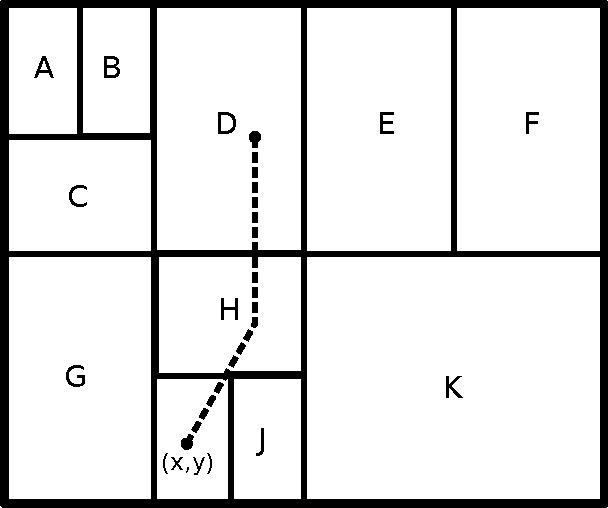
\includegraphics[scale=0.4]{img/algorithms/landmark_binning}
\caption{Example 2D coordinate overlay and a sample routing path from node D to
(x,y).}
\label{fig:landmark_binning}
\end{figure*}
Landmark Binning \cite{ratnasamy_binning_2002} is an approach to partition close
by nodes into bins based on their distance to well known anchor nodes across the
Internet, as shown in Figure \ref{fig:landmark_binning}. In order to detect
locality, nodes use network latency (i.e. RTT) as a measurement technique. The
network latency, even though not always accurate, is selected in this work due
to its non-intrusive, transparent and easy to apply behaviour. In order for the
binning to work, few well known anchor servers with known physical locations on
the Internet. Authors estimate that a number of 12 such servers can prove
sufficient for this. The nodes measure their distance to all these servers and
record the latency values for each. Later, the tuple of these latency values
represents the bin of each node. Nodes with similar latency values are
considered close to each other, or at least within the same autonomous system.
The operation of the method is independent of the model incorporated by the
overlay network and thus it can be applied with no significant changes to both
structured and unstructured P2P systems. \cite{ratnasamy_binning_2002} has the
detailed description of such algorithm for both architectures. Landmark binning
is also considered as a good candidate for content distribution networks in
particular. The major disadvantage of landmark binning is to install and
maintain landmark servers on different autonomous systems, all over the world.
A typical P2P network usually has a couple of million nodes connected at any
given time, thus rendering landmark servers an important parameter when
designing for large scales.  The authors claim that latency estimation does not
drain much from the network resources but in case scalability problems arise,
they claim the solution is replacing single landmark servers with clusters of
servers within the same physical area. However, this approach does not reduce
the possibility of excessive network traffic flow through these landmark
servers. One other possible problem is the incorrect binning caused by the use
of inaccurate methods for delay measurement, since tracking down, for example,
network latencies is far from proven to be safe for location estimation.

% TODO: MAYBE THANCS deserves some more attention here

\paragraph*{\bf mOverlay}
mOverlay \cite{zhang_moverlay_2004} tries to addresses the scalability
issues that might be imposed to networks when using static landmark servers by
introducing the dynamic landmarks. The authors introduce the notion of a group
which is a set of  peer considered close to each other with respect to any
position in the underlying network, proximity being some  user-defined cost
metric (i.e. round-trip-time). mOverlay, tries to recreate small-world-like
properties to the overlay network by creating a a two-level hierarchical
structure, where on the top level we have connections between groups while on
the bottom we have connections between peers inside groups. Finding the correct
closest group is the most important part  of the overlay construction. Nodes are
grouped based on their  distance to the groups already in the network, rendering
the  later the (dynamic) landmarks for the process. The authors formally prove
that any new node can reach its group by exchanging at most $O(logN)$ messages
within the network. Finally mOverlay also considers a second important function
in its protocol which is the constant maintenance of the overlay.

\renewcommand\arraystretch{1.4}% (MyValue=1.0 is for standard)

%\begin{figure}[h!]
\hspace{-3ex}
\begin{center}
\footnotesize
%\begin{tabular}{
%\begin{landscape}
\begin{longtable}{
|>{\columncolor[gray]{.7}}m{0.2\columnwidth}
|>{\columncolor[gray]{.9}}m{0.4\columnwidth}
|>{\columncolor[gray]{.8}}m{0.2\columnwidth}
|>{\columncolor[gray]{.9}}m{0.2\columnwidth}
%|>{\columncolor[gray]{.9}}m{0.1\columnwidth}
%|>{\columncolor[gray]{.8}}m{0.1\columnwidth}
%|>{\columncolor[gray]{.9}}m{0.1\columnwidth}
%|>{\columncolor[gray]{.8}}m{0.1\columnwidth}
|}
\caption{Decentralized Unstructured Algorithms} \label{fig:unstruct_compare_table} \\
\hline
\rowcolor[gray]{.5}
\textbf{Algorithm} &  \textbf{Overlay structure} & \textbf{Base protocol} &
 \textbf{Scalability}\\
\hline
\endfirsthead
\multicolumn{4}{c}%
{\tablename\ \thetable\ -- \textit{Continued from previous page}} \\
\hline
\rowcolor[gray]{.5}
\textbf{Algorithm} &  \textbf{Overlay structure} & \textbf{Base protocol} &
 \textbf{Scalability}\\
\hline
\endhead
\hline \multicolumn{4}{r}{\textit{Continued on next page}} \\
\endfoot
\hline
\endlastfoot
\textbf{Narada} & \textbf{Overlay optimization
based}. Creates a mesh (richer connected graph) and builds minimum spanning
trees on this mesh & & Small and sparse groups \\

\hline
\textbf{Gia} & \textbf{Broadcast based} Replaces
Gnutella flooding with random walk, and introduces KaZaA style supernodes. Uses
dynamic topology adaptation protocol &
 Gnutella &  Better than Gnutella  \\

\hline
\textbf{Adaptive Overlay Topology Optimization} & \textbf{Overlay optimization
based}. Creates overlay multicast tree with Selective Flooding protocol&
Gnutella &  Better than Gnutella \\

\hline
\textbf{Location-aware Topology Matching} &
\textbf{Overlay Optimization Based}. Uses \textit{TTL2-detector flooding}, \textit{low productive
connection cutting}, and \textit{source peer probing}. & Gnutella &  Better than Gnutella \\

\hline
\textbf{Replication Strategies in Unstructured P2P Networks} &
\textbf{Cache Based}. Uses uniform, proportional and square root allocation
strategies to replicate data. & Gnutella &  Better than Gnutella \\

\hline
\textbf{Tracing a large-scale Peer to Peer System: an hour in the life of Gnutella.} &
\textbf{Cache Based}. Proposes a caching algorithm based on the traces of the Gnutella traffic & Gnutella & Better than Gnutella \\

\hline
\textbf{Improving search in P2P networks} &
\textbf{Broadcast Based}. Uses \textit{iterative deepening}, \textit{directed
BFS}, and \textit{local indices} to improve efficiency. & Gnutella &  Better than Gnutella \\

\hline
\textbf{Distributed Cycle Minimization Protocol} &
\textbf{Broadcast based} Uses a decentralized cycle elimination protocol  &  &  \\

\hline
\textbf{Scalable Bipartite Overlay} &
\textbf{Overlay optimization based} Uses bipartite partition graph and builds
local minimum spanning trees  & Gnutella  & Better than Gnutella \\

\hline
\textbf{Adaptive Connection Establishment} &
\textbf{Overlay optimization based} Forms Neighbour Cost Tables, builds local
minimum spanning trees and perform local optimizations & Adaptive Overlay
Topology Optimization (AOTO), Gnutella & Better than Gnutella \\

\hline
\textbf{Hops Adaptive Neighbour Discovery} &  & &  \\

\hline
\textbf{Two-Hop-Away Neighbour Comparison and Selection (THANCS)} &
\textbf{Overlay optimization based} Uses piggybacking to discover neighbour
distances and selects neighbours  & Gnutella  & \\

\hline
\textbf{mOverlay} &\textbf{Landmark based proximity} Uses dynamic landmarks to find node locality
& & Due to dynamic landmarks and grouping, more scalable than tree-based or mesh-based protocols \\

\hline
\textbf{Distributed Domain Name Order (DDNO)} &
\textbf{Overlay optimization based} Connects half of the nodes connections to
the nodes in the same domain and the other half to random nodes, therefore
supports locality and topological connection  &  & Yes, by using super
peers \\

\hline
\textbf{Peer-exchange Routing Optimization Protocols} & \textbf{Overlay optimization based} Optimizes overlay by the exchange of
neighbors among peers  & Can work with both decentralized structured and
unstructured architecture & Yes \\

\hline
\textbf{MAY OMIT- T2MC} &
\textbf{Overlay optimization based} Uses traceroute results for clustering the
nodes  & & \\

\hline
\textbf{Unnamed-unstructured} &
\textbf{Overlay optimization based} Minimizes the communication delay and
maximizes the broadcasting range & & Better than THANCS and mOverlay \\

\hline
\textbf{Landmark Binning} & \textbf{Landmark based proximity} Uses network latency to partition
nodes into bins & Can work with both decentralized structured and unstructured architecture & \\

\hline
%\end{tabular}
\end{longtable}
%\end{landscape}
\end{center}
\vspace{-2.5ex}
\vspace{-2.5ex}
%\end{figure}

%%%%%%%%%%%%%%%%%%%%%%%%%%%%%%%%%%%%%%%%%%%%%%%%%%%%%%%%%%%%%%%%%%%%%%%%%%%%%%%%
%%%%%%%%%%%%%%%%%%%%%%%%%%%%%%%%%%%%%%%%%%%%%%%%%%%%%%%%%%%%%%%%%%%%%%%%%%%%%%%%
\subsection{Discussion on the Algrithms for Unstructured Architectures}
%%%%%%%%%%%%%%%%%%%%%%%%%%%%%%%%%%%%%%%%%%%%%%%%%%%%%%%%%%%%%%%%%%%%%%%%%%%%%%%%
%%%%%%%%%%%%%%%%%%%%%%%%%%%%%%%%%%%%%%%%%%%%%%%%%%%%%%%%%%%%%%%%%%%%%%%%%%%%%%%%

In this section we presented the state of the art for the algorithms applied to
unstructured P2P systems. We categorised it based on their philosophy for
alleviating the topology mismatch problem into four major categories namely
\begin{inparaenum}[\itshape i\upshape)]
  \item broadcast-based,
  \item cache-based,
  \item overlay optimisation-based and
  \item landmark-based approaches
\end{inparaenum}
. Here we present a overall discussion on the above categories trying to point
out the advantages, disadvantages and novelties introduced by each and by all of
them. A quick overview can be seen in Table \ref{fig:unstruct_compare_table}.

Broadcast-based approaches in general propose intelligent neighbour selection in
order to replace the inefficient blind flooding first used in the Gnutella
protocol. Instead of forwarding the queries to all their outgoing links they
dictate the intelligent selection of neighbours with either higher probability
to answer a query than others or neighbours  that expose specific features such
as high bandwidth, high capacity, or low latency. This, in practice reduces the
aggregate resource usage of the P2P network and improves the overall performance
of the system. On the other hand, the algorithms do not offer a real solution to
the topology mismatch problem. Thus, none can guarantee that overlay and
underlying topologies are aligned with each other let alone quantify the
mismatch and try to alleviate. Broadcast-based methods can be used in
conjunction with other approaches to improve the quality of the P2P systems.

The success of caching, as a well studied method in client-server Internet
applications, also made it a good candidate for the P2P networks. Even
though caching improves the performance, and reduces the overall resource usage
of P2P systems, the design of caches in this context is non-trivial compared to
the web-based caching. Due to the unique, inherent characteristic of all P2P
systems that, each node can act as both a server and a client, two important
issues have to be considered when designing caches. First, the lifetime of a
query is short, as the nodes join and leave frequently. Second, the result of a
single query string is not always the same, as it is dependent on the source of
the query, the TTL value set for the messages, the current interconnection of
peers and the high volatility of the environment. So, in order to develop a
successful caching system for a P2P architecture, these parameters also have to
be considered. Even though the state of the art P2P algorithms using caching
methods reduce the resource usage of the network, they also fail to consistently
address the probelem of the topology mismatch.

Overlay-optimisation-based  can further be devided into
minimum-spanning-tree-based and clustering-based. Researchers initially started
considering alternatives to IP multicast for the application layer, which led
Narada, that simulates the same one-to-many communication approach requiring IP
multicast services. Application layer multicast, however, is not as efficient as
the one enabled by IP and still struggles to ease the difficulties imposed by
the topology mismatch problem. Narada, and its followers (AOTO, LTM, SBO) try to
solve the topology mismatch problem by building a richer connected graph and
forming minimum spanning trees over this graph that can efficiently route
messages among peers. Application level multicast protocols, pioneered by
Narada, are generic protocols that can be applied to both P2P file sharing
systems, as well as content distribution networks. The original Narada algorithm
is designed for small groups therefore it is not scalable. Its followers try to
solve the scalability problem by introducing various methods including forming
minimum spanning trees for the two-hop neighbours ($N^2$) of each node,
partitioning the graph into two random groups where each group is responsible of
different tasks, or performing local optimizations dynamically on the overlay
graph. The advantage of building minimum spanning trees is that they maintain
the connectivity on the network in an efficient manner, while still preserving
the overall search scope. However, building and maintaining a minimum spanning
tree creates additional overhead for the network. The alternative method used in
overlay optimization is the cluster based approache. According to that, nodes
use various methods to detect physically close nodes to form clusters. T2MC uses
traceroute logs and DDNO uses domain names to cluster close by nodes. However,
the accuracy of the methods used to form clusters directly affect the success
rate of the algorithm. Traceroute for example is a heavy weight utility to be
frequently used on the network, let alone the fact that many network equipment
vendors do not allow traceroute calls. The major problem with cluster based
approaches is that the limited connectivity within the local domains shrink the
search scope dramatically, which negatively affects the search performance of
the P2P system. DDNO addresses this limitation by allowing half of each nodes
connections to be to random nodes over the network, which balances the
efficiency of the clustering approach with improved connectivity.

In landmark-based algorithms, nodes use network delay (e.g. RTT) as a
distance measurement method to position themselves with respect to ``a priori''
known servers (the landmark servers) on the Internet. Landmark servers are used
by nodes to estimate their positions based on the intutive assumption that nodes
with similar distances to a set of landmarks, are physically close to each
other, as well, over the network. The landmark based protocol has two important
drawbacks. Firstly the network delay is not a reliable distance estimation
method. For example, based on the load on the network the delay to certain nodes
or networks can change from time to time, which will eventually affect the
distance measurements and wrong measurements will lead to wrong estimated
positions for the nodes, or incorrect and non optimal clusterings of the nodes.
The second drawback of using landmark servers is the cost of installing and
maintaining this kind of infrastructure across the whole Internet and for all
the different autonomous system domains. As popular P2P file sharing
applications usually have millions of peers connected at any time, it is not
false to assume that the network costs of maintaining these landmark servers
will be quite high. A possible solution to the scalability problem of the static
landmark servers is to use ordinary nodes as dynamic landmarks once they
estimate their own positions. Even though this approach scales much better than
static landmark servers, still the measurement accuracy problem affects the
overall performance of the system.